\section{Inverting Amplifier}
\subsection{Pengantar Inverting Amplifier}
\begin{frame}{Pengantar Inverting Amplifier}
	\begin{itemize}
		\item Inverting amplifier: rangkaian op amp paling dasar
		\item Menggunakan negative feedback untuk menstabilkan keseluruhan voltage gain
		\item Keseluruhan voltage gain perlu distabilkan karena $ A_{VOL} $ sangat besar dan tidak stabil
		\item 741C memiliki $ A_{VOL} $ minimum sebesar 20000 dan $ A_{VOL} $ maksimum lebih dari 200000
	\end{itemize}
\end{frame}

\subsection{Inverting Negative Feedback}
\begin{frame}{Inverting Negative Feedback}
	\begin{figure}
		\centering
		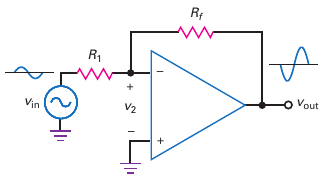
\includegraphics[height=0.5\textheight]{gambar/fig-16.12}
		\caption{Inverting amplifier}
		\label{fig-16.12}
	\end{figure}
\end{frame}

\subsection{Virtual Ground}
\begin{frame}{Virtual Ground}
	\begin{figure}
		\centering
		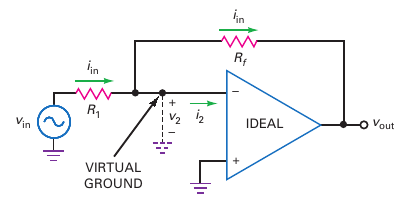
\includegraphics[height=0.5\textheight]{gambar/fig-16.13}
		\caption{Konsep virtual ground}
		\label{fig-16.13}
	\end{figure}
\end{frame}

\subsection{Voltage Gain}
\begin{frame}{Virtual Ground}
	\begin{figure}
		\centering
		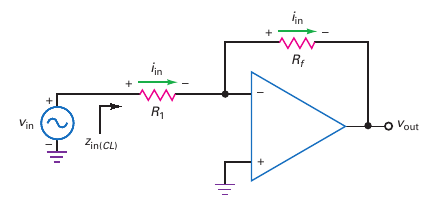
\includegraphics[height=0.5\textheight]{gambar/fig-16.14}
		\caption{Inverting amplifier memiliki arus yang sama yang melewati kedua resistor}
		\label{fig-16.14}
	\end{figure}
\end{frame}

\subsection{Bandwidth}
\begin{frame}{Bandwidth}
	\begin{multicols}{2}
		\begin{figure}
			\centering
			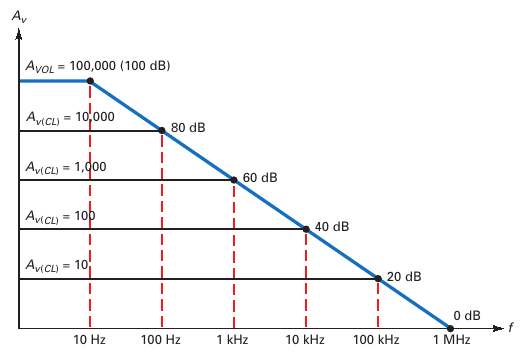
\includegraphics[height=0.6\textheight]{gambar/fig-16.15}
			\caption{Voltage gain yang lebih kecil menghasilkan bandwidth yang lebih besar}
			\label{fig-16.15}
		\end{figure}
	\columnbreak
		\begin{itemize}
			\item 
		\end{itemize}
	\end{multicols}
\end{frame}